Ergodic literature should leave you wondering whether or not you've even read it all.

\href{/map}{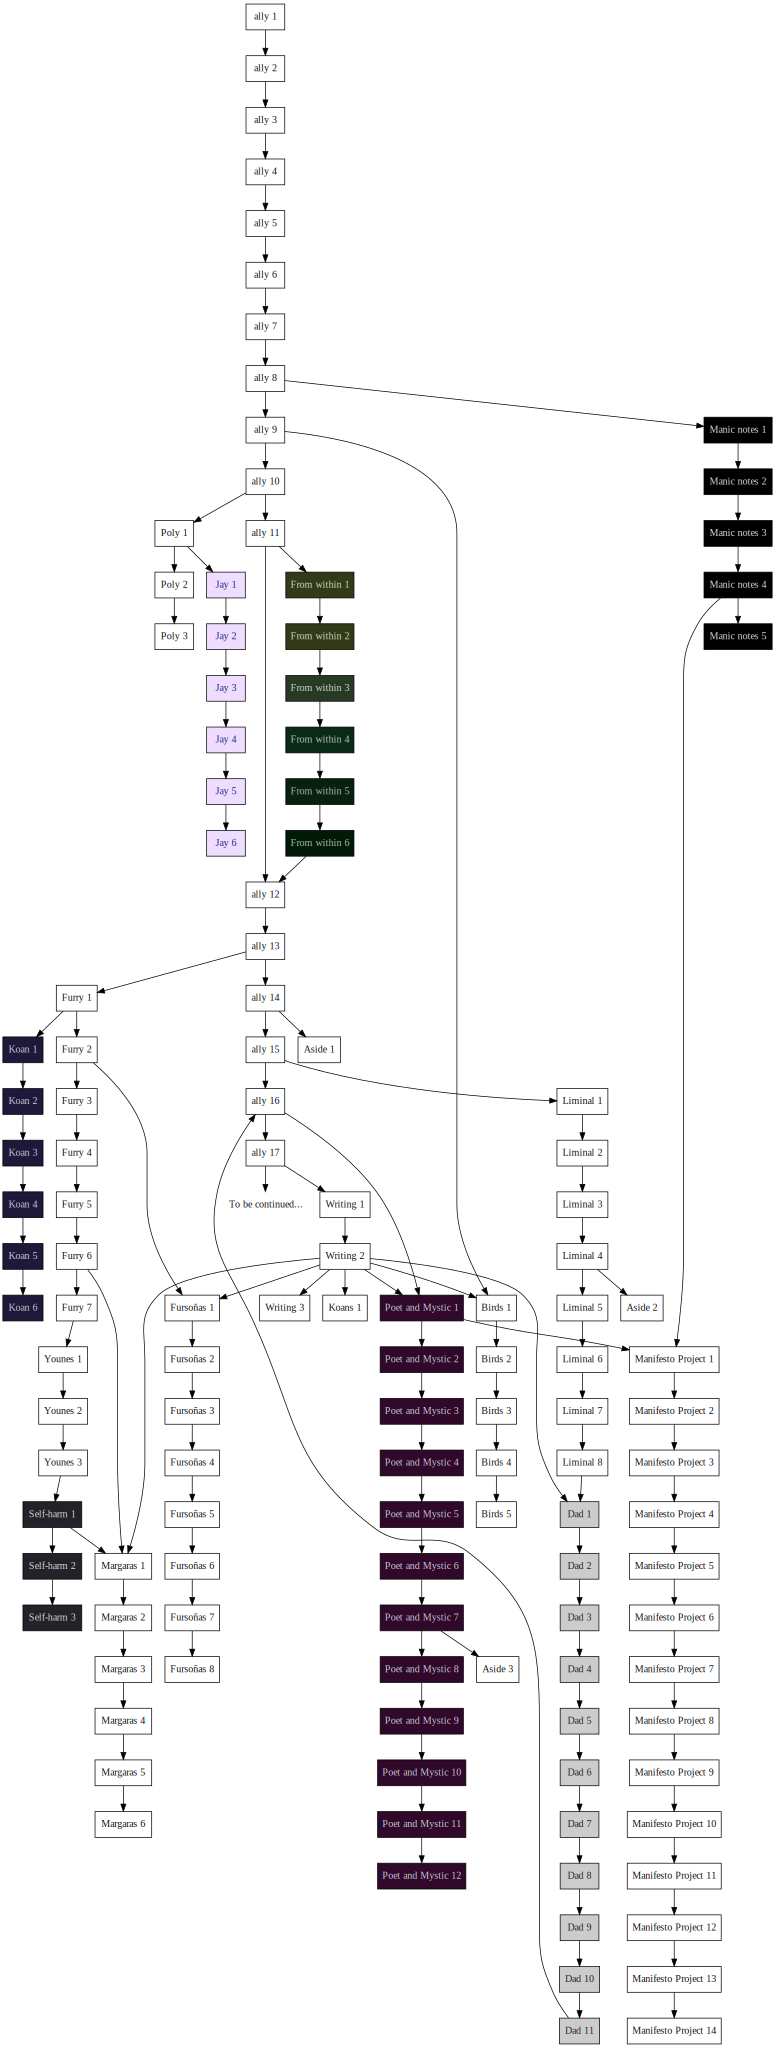
\includegraphics{/map.png}}

This big reorganization intentionally makes the project far less linear and, in a way, more difficult to navigate. Ergodic literature takes work. Hypertextual art should be truly hypertextual.

\begin{quote}
Countdown to Maddy including transclusion.
\end{quote}

Don't tempt me.

As an affordance for this increased difficulty, I'll be providing news updates with each content update stating what's been added or changed.

\hypertarget{new-content}{%
\subsection{New content}\label{new-content}}

\begin{itemize}
\tightlist
\item
  \href{/writing}{Writing 1}
\item
  \href{/writing/2}{Writing 2}
\item
  \href{/writing/3}{Writing 3}
\end{itemize}
